\documentclass[a4paper,12pt]{article}
\usepackage[utf8x]{inputenc}
\usepackage{amssymb}
\usepackage{amsfonts}
\usepackage{mathrsfs}
\usepackage{amsmath}
\usepackage{amsthm}
\usepackage[margin=3cm]{geometry}
\usepackage{times}
\usepackage{graphicx}
\usepackage{enumitem}
\usepackage{fancyhdr}
\usepackage{hyperref}
\usepackage{setspace}
\usepackage{subcaption}
\usepackage{mathtools}

\pagestyle{fancy}
\fancyhf{}
\lhead{Thomas Delaney}
\rhead{Fluorescence Modelling}
\cfoot{\thepage}

\newtheorem{theorem}{Theorem}
\newtheorem{proposition}{Proposition}[section]
\newtheorem{lemma}{Lemma}[section]
\newtheorem{corollary}{Corollary}[section]
\theoremstyle{definition}
\newtheorem{definition}{Definition}[section]

\newcommand{\boldnabla}{\mbox{\boldmath$\nabla$}} % to be used in mathmode
\newcommand{\cbar}{\overline{\mathbb{C}}}% to be used in mathmode
\newcommand{\diff}[2]{\frac{d #1}{d #2}}% to be used in mathmode
\newcommand{\difff}[2]{\frac{d^2 #1}{d #2^2}}% to be used in mathmode
\newcommand{\pdiff}[2]{\frac{\partial #1}{\partial #2}} % to be used in mathmode
\newcommand{\pdifff}[2]{\frac{\partial^2 #1}{\partial #2^2}}% to be used in mathmode
\newcommand{\upperth}{$^{\mbox{\footnotesize{th}}}$}%to be used in text mode
\newcommand{\vect}[1]{\mathbf{#1}}% to be used in mathmode
\newcommand{\curl}[1]{\boldnabla \times \vect{#1}} % to be used in mathmode
\newcommand{\divr}[1]{\boldnabla \cdot \vect{#1}} %to be used in mathmode
\newcommand{\modu}[1]{\left| #1 \right|} %to be used in mathmode
\newcommand{\brak}[1]{\left( #1 \right)} % to be used in mathmode
\newcommand{\comm}[2]{\left[ #1 , #2 \right]} %to be used in mathmode
\newcommand{\dop}{\vect{d}} %to be used in mathmode
\newcommand{\cov}{\text{cov}} %to be used in mathmode
\newcommand{\var}{\text{var}} %to be used in mathmode
\newcommand{\mb}{\mathbf} %to be used in mathmode
\newcommand{\bs}{\boldsymbol} %to be used in mathmode
% Title Page
\title{Modelling the fluorescence produced by fluorescent calcium indicators in response to sequences of action potentials}
\date{}
\author{Thomas J. Delaney \\ Cian O'Donnell, Michael C. Ashby}

\begin{document}

\maketitle

\newpage

\abstract{The use of fluorescent calcium indicators, such as GCaMP6s, to monitor neuronal activity is widespread. But the relationship between the fluorescence signal and action potential firing is poorly understood. Furthermore, the effects of the indicator characteristics on this fluorescence signal are unknown. For example, it is known that genetically encoded indicators accumulate within neurons over weeks and months. This makes comparison of activity levels at different time points difficult. As a result, whether or not spike train inference is always possible using fluorescent calcium indicators remains unknown.

The aim of this project was to model the fluorescence traces produced by a fluorescent calcium indicator in a neuron soma, given parameters such as binding rate, dissociation rate, and molecular concentration from a specific spike train. The ultimate goal of the model is to allow benchmarking of the various spike inference algorithms that have been developed, and to understand how indicator characteristics affect the quality of spike train inference.

The modelled cell contents consisted of free calcium, fluorescent indicator molecules, and mobile and immobile endogenous calcium buffers. The indicator molecules which were bound to a calcium molecule could be either excited, i.e. able to release a photon, or relaxed. In order to reproduce the noise in the system dynamics, we modelled the release of photons from the excited indicator bound calcium as a stochastic process.

The fluorescence traces produced by the simulation were calibrated to reproduce the signal-to-noise ratio observed in experimental data. Spike inference algorithms were used to infer spike trains from the experimental fluorescence traces and the modelled fluorescence traces. The parameters of the model were then varied in order to determine the effect on the system dynamics and the effects on spike inference.} % no citations in the abstract

\newpage

\tableofcontents

\newpage

\section{Introduction}
\subsection{Fluorescent calcium indicators}
Since the invention of two-photon calcium imaging, the use of fluorescent calcium indicators to study the activity of populations of neurons has grown in popularity. In this process, the neurons are made to fluoresce using one of three methods. Either a calcium sensitive dye is injected into the body of each cell to be monitored, or the cells are altered by a virus, or the cells are genetically modified to make them express a calcium sensitive protein. The dye or the proteins fluoresce when they come into contact with and bind to calcium molecules. This fluorescence allows us to locate the cells containing the fluorescent indicator. Furthermore, since the firing of an action potential involves an influx of calcium molecules, the indicator makes the firing of action potentials observable by an increase and subsequent decay in fluorescence inside the cell. An example of the fluorescence produced by a fluorescent calcium indicator can be seen in figure \ref{fig:GCaMP6_fluorescence}. The activity of the cell is quantified by measuring $\Delta F/F_0 = (F - F_0)/F_0$, where $F$ is the fluorescence within the soma, and $F_0$ is the baseline fluorescence within the soma \cite{maravall}. The fluorescence traces that make up the data used in this research are just measurements of $\Delta F/F_0$ at each time step. An example trace can be seen in figure \ref{fig:spike_finder_example}.

\begin{figure}[ht]
  \centering
  \includegraphics[width=0.9\textwidth]{figures/GCaMP6_fluorescence.png}
  \caption{Single frame from video of spontaneous activity recorded from cultured mouse hippocampal neurons using GCaMP6s fluorescent indicator. Image courtesy of brainslicemethods.com}
  \label{fig:GCaMP6_fluorescence}
\end{figure}

Calcium imaging has a number of advantages over the more traditional electrophysiological methods. Firstly, electrophysiological methods involve inserting a electrode or a number of electrodes into the brain to measure extra-cellular voltages. The electrodes need to be attached by wires to a device that collects their data. This inhibits the movement of the experimental subject, and makes longitudinal experiments impossible. The calcium imaging can be performed \textit{in vivo} \cite{stosiek}, and the apparatus can be removed from the subject when the subject is not under observation. This enables longitudinal experiments as the subject can survive and move around normally when not being examined. Furthermore, inserting these electrodes can cause cells, or the connections between cells to be damaged. Using calcium imaging avoids this kind of damage. Also, in electrophysiology, the strength of the spiking signal, and the position of each electrode are used by purpose designed algorithms to identify the position of individual neurons and ‘sort’ the spikes, i.e. attribute the spikes to a cell. This method is very good for spike detection and attribution. But these methods are biased toward readings from the most active cells. In fact, an inactive cell will be completely ignored by electrophysiological methods. With calcium imaging, inactive cells are still detected since each cell contains a baseline level of calcium \cite{maravall}, and therefore fluorescences a small amount. Finally, electrophysiological methods can only read from the cells nearby the electrodes. Genetically encoded fluorescent calcium indicators such as GCaMP6s can be targeted at neurons with a specific genetic make-up.

fMRI methods can also be used to monitor brain activity. But the resolution is too low to monitor individual cells.

\begin{figure}[p]
  \begin{subfigure}{\textwidth}
    \centering
    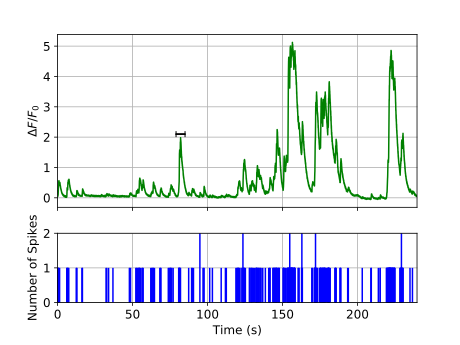
\includegraphics[width=0.9\textwidth]{figures/spike_finder_example_8.png}
    \caption{Plot of a spike train and the corresponding GCaMP6s fluorescence trace. Data courtesy of spikefinder.codeneuro.org}
  \end{subfigure}
  \begin{subfigure}{\textwidth}
    \centering
    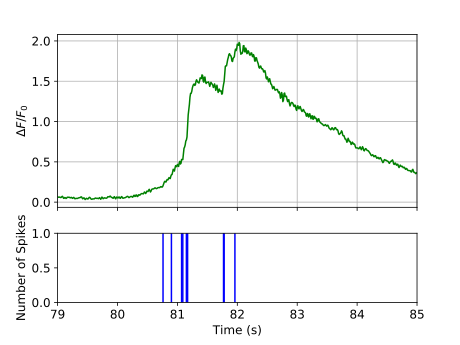
\includegraphics[width=0.9\textwidth]{figures/spike_finder_example_8_zoomed.png}
    \caption{The same image as (a) but zoomed into the period from 80s to 86s. A group of six action potentials around the 81s point followed by a group of three action potentials just before the 82s point are shown. The decay of the fluorescence trace is much slower than the dynamics of an action potential.}
  \end{subfigure}
  \caption{}
  \label{fig:spike_finder_example}
\end{figure}

There are some drawbacks to fluorescent calcium indicators. For example, the dynamics of the fluorescent indicators are much slower than the dynamics of action potentials. After excitation, the cross-membrane potential of a cell will return to baseline in $2-3$ms. After a single action potential, the fluorescence of GCaMP6s will return to baseline after approximately $3$s. At least a thousand times longer. An example of this can be seen in a figure \ref{fig:spike_finder_example}, showing a fluorescence trace and the corresponding spike train. The relaxation time is extended when more than one action potential is fired in quick succession \cite{chen}. These slower dynamics make it difficult to infer exact spike times and to infer how many spikes occurred in a given time period. For some research it is sufficient to use $\Delta F/F_0$ as measure of cell activity. But if spike timing is an important factor, then this drawback of fluorescent indicators should be taken into account. Also, we should bear in mind that neurons communicate with each other using action potentials, not fluorescence signals.

Fluorescence readings are usually taken from cells after a `loading period', so that the indicator is saturated within the cells. At this point the increase in fluorescence in response to an action potential will be greatest. So another issue with the genetically encoded indicators is that it is impossible to know whether or not the indicator is saturated within the cell. This is especially a problem with longitudinal studies, as the amplitude of fluorescence change in response to an action potential, and the baseline fluorescence $F_0$, will change as the experiment continues. This means that the same amount of activity in cells will give different values for $\Delta F/F_0$ at different times, which makes analysis difficult. It is claimed that despite this it is still possible to detect individual spikes, even in spike bursts \cite{chen}.

In this project we aim to make a model, which given a spike train and some parameters defining the characteristics of a calcium indicator, will return the fluorescence trace induced by this spike train. Our aim with this model is to provide a way of assessing what effect changes in indicator characteristics will have on the fluorescence traces. This tool should prove useful for experimentalists in setting up their experiments. It should be also be useful for anyone who wants to create some simulated calcium imaging data.

\subsection{Spike Inference Algorithms}
There are existing methods for converting the fluorescence traces into spike trains \cite{vogelstein, pnevmatikakis, jewell, friedrich}, but these methods have not been tested rigorously. Also, these methods do not take experimental variations into account, such as a variation in the concentration of the indicator. Furthermore, the process of collecting the photons emitted by the indicator introduces some noise. Whether or not this noise is enough to obfuscate the spiking signal has never been investigated. Our model should help to assess whether or not it is possible to infer spike trains accurately. It should also be possible to compare the performance of difference spike inference algorithms using this model.

\section{Methods \& Data Sources} % description of everything used to create the results, and justifications for assumptions/approaches/parameters

\subsection{Modelling}\label{sec:model}

\subsubsection{Calcium Dynamics}\label{sec:calcium_dynamics}
When a neuron fires an action potential, voltage-dependent calcium ion-channels open up that allow a current of Ca$^{2+}$ to flow into the neuron \cite{koch}. The increase in the free calcium ion concentration inside of the cell along with changes in the concentration of potassium and sodium causes the change in cell membrane potential, which must be depolarised. The depolarising process consists of free calcium ions leaving the cell through open ion channels, binding to molecules within the cell called \textit{buffers}, and some calcium storage by organelles such as the endoplasmic reticulum. A diagram illustrating the cell, its channels, and its buffers can be seen in figure \ref{fig:cell_diagram} There are several different types of calcium buffer, each with different dynamics and different concentrations within different types of excitable cell. The fluorescent calcium indicator is another calcium buffer, with the useful property that when it is bound to a calcium ion, the bound molecule may become excited by a photon and release a photon in return. This is what creates the fluorescence. After the action potential has taken place, the free calcium concentration within the cell will return to a baseline level \cite{maravall}.

\begin{figure}[h]
  \centering
  \includegraphics[width=0.7\textwidth]{figures/cell_diagram.png}
  \caption{A diagram showing the methods by which Ca$^{2+}$ can enter the cell, leave the cell, and become `buffered'.}
  \label{fig:cell_diagram}
\end{figure}

\subsubsection{The Model}\label{sec:the_model}
We modelled the the dynamics of five molecular concentrations within the body of a neuron,
\begin{itemize}
  \item Free calcium ion concentration, $[Ca^{2+}]$,
  \item Fluorescent indicator bound calcium, $[BCa]$,
  \item Endogenous mobile buffer bound calcium, $[ECa]$,
  \item Endogenous immobile buffer bound calcium, $[ImCa]$,
  \item Excited buffered calcium, $[BCa^*]$.
\end{itemize}
The term `buffering' refers to free calcium ions coming into contact with buffer molecules and binding together. Diagrammatically this is:
\begin{equation*}
   [X][Ca^{2+}] \xrightleftharpoons[k_{Xb}]{k_{Xf}} [XCa]
\end{equation*}
where $[X]$ represents any buffer molecule, and $k_{Xf}$ and $k_{Xb}$ represent the binding and unbinding (dissociation) rates in units of per molar concentration per second ($M^{-1}s^{-1}$) and per second ($s^{-1}$) respectively. The speed of this chemical reaction is determined by the binding and unbinding rates.

There are a number different endogenous buffers in any neuron. Which buffers are present, and the buffers' concentrations vary from cell to cell. In order to capture the effects of mobile and immobile endogenous buffers without introducing several parameters they were modelled as two buffers. One representing mobile buffers and the other representing immobile buffers. Each with their own binding and unbinding rates.

The fluorescent calcium indicator behaves similarly to the other calcium buffers. The calcium is buffered by the indicator in the same way. But an indicator bound calcium molecule can become excited by absorbing the energy from a photon. An excited indicator bound calcium molecule can then release a photon to go back to its `relaxed' state.
\begin{equation*}
   [B][Ca^{2+}] \xrightleftharpoons[k_{Bb}]{k_{Bf}} [BCa] \leftrightsquigarrow [BCa^{*}]
\end{equation*}
The released photons are captured by a photon collector. This gives us the fluorescence trace.

Ignoring the baseline level of free calcium in a neuron, the system of equations we used to model all of these interactions is as follows:
\begin{equation} \label{eq:model_equations}
  \begin{split}
  \diff{[Ca^{2+}]}{t} = & k_{Bb}[BCa] + k_{Eb}[ECa] + k_{Imb}[ImCa] \\
                      & - k_{Bf}[B][Ca^{2+}]- k_{Ef} [E][Ca^{2+}] - k_{Imf}[Im][Ca^{2+}] \\
                      & + \beta ([Ca^{2+}_{0}] - [Ca^{2+}])
  \end{split}
\end{equation}
\begin{align}
  \diff{[BCa]}{t} = & k_{Bf}[B][Ca^{2+}] - k_{Bb}[BCa] + r[BCa^{*}] - e[BCa] \\
  \diff{[ECa]}{t} = & k_{Ef}[E][Ca^{2+}] - k_{Eb}[ECa] \\
  \diff{[ImCa]}{t} = & k_{Imf}[Im][Ca^{2+}] - k_{Imb}[ImCa] \\
  \diff{[BCa^{*}]}{t} = & e[BCa] - r[BCa^{*}]
%  \end{split}
\end{align}
where $[Ca^{2+}_{0}]$ is the baseline calcium concentration within the cell soma, $\beta$ is a rate defining how quickly free calcium enters or leaves the cell in the absence of an action potential, $e$ is the excitation rate for indicator bound calcium, $r$ is the photon release rate for the excited indicator bound calcium, and $f$ and $b$ are used to indicate the forward and backward rates for chemical reactions respectively. The excitation rate defines the proportion of indicator bound calcium that becomes excited at each time step. The photon release rate defines the proportion of excited indicator bound calcium that releases a photon and returns to its relaxed state at each time step. An action potential is modelled as a discontinuous increase in the free calcium concentration to an appropriate value \cite{maravall}.

Note that each of the three pairs of binding and unbinding terms in the first equation has a corresponding pair in one of the subsequent three equations. Binding removes a free calcium molecule and adds a bound calcium molecule, and unbinding does the opposite. Note that the excitation and release dynamics are included by the last two terms in the equation $4$, and all of equation $7$. The last term in equation $1$ drives the free calcium concentration back to the baseline level $[Ca^{2+}_{0}]$. The calcium rate, $\beta$, controls how quickly the concentration will be driven to the baseline.

When using this model to simulate a fluorescence trace, the system of equations above are first solved over a period of $25$s in the absence of any action potentials. This lets each of the five tracked chemical concentrations to reach their steady state, before using the given spike train and the given parameters to model the fluorescence trace.

Note that since the model has no spatial component, the mobile and immobile buffers only differ in their binding and unbinding rates.

\subsubsection{Photon release \& capture}\label{sec:photon_capture}
We used a simple model for the photon release. The number of photons released at each time step was controlled by the number of excited indicator bound calcium molecules in the cell and a parameter called the `release rate'. The release rate is an optimised free parameter of the model.

As for the photon capture, in two-photon excitation microscopy the photons scattered by the fluorescent indicator get scattered in all directions. Therefore the number of photons detected is stochastic. This made the process for capturing photons the natural source of noise in the system. The number of photons captured, and therefore the intensity of the fluorescence, is modelled using a binomial distribution.

A binomial distribution is the discrete probability distribution of the number of successes in a sequence of independent trials with a binary outcome. The parameters defining the distribution are:
\begin{itemize}
  \item $n$, The number of trials
  \item $p$, The probability of success
\end{itemize}
The probability mass function of the distribution is
\begin{equation}
  Pr(\text{number of successes} = k) = {{n}\choose{k}}p^k(1-p)^{n-k}
\end{equation}

The number of photons released was used as number of trials. This was a natural choice as each photon is either captured, or not captured. The probability of success is set equal to the `capture rate'. The capture rate is a free parameter of the model to be optimised.

\subsubsection{Parameter optimisation} \label{sec:opt_params}
The free parameters of the model are as follows:
\begin{description}
  \item[Calcium rate, $\beta$] Controls how quickly the concentration of free calcium will be driven to the baseline concentration.
  \item[Capture rate, $p$] The average proportion of photons captured by the photon detector.
  \item[Excitation rate, $e$] The number of indicator bound calcium molecules that become excited by photon bombardment at each time step.
  \item[Release rate, $r$] The number of excited indicator bound calcium molecules that release a photon at each time step.
\end{description}
To optimise the free parameters given a fluorescence trace, we applied the following procedure:
\begin{enumerate}
  \item The frequency power spectrum of the trace was measured.
  \item The power spectrum was smoothed using a boxcar smoother (aka. sliding average, box smoother).
  \item The log of the smoothed power spectrum was measured.
  \item Use the model to create a modelled fluorescence trace
  \item Apply steps 1, 2, and 3 to the modelled fluorescence trace.
  \item Calculate the root mean squared difference between the log power of the actual fluorescence trace, and the log power of the modelled fluorescence trace.
  \item Calculate the root mean squared difference between the actual fluorescence trace and the modelled fluorescence trace.
  \item Use an optimisation algorithm to reapply this process, attempting to minimize the sum of the two root mean squared differences at each iteration.
\end{enumerate}
Using the root mean squared difference of the log power spectra as part of the objective function forces the model to match the noise frequency of the actual fluorescence. Using the root mean squared difference of the traces themselves forces the model to match the amplitude of the fluorescence changes more accurately. % (Should I be saying this???)

In order to minimise the objective function, a suite of \textit{meta-heuristic optimisation} (aka. \textit{black-box optimisation}) algorithms were implemented on each of the traces in the dataset. These methods were chosen because they don't require a gradient for the objective function (gradient-free) and they are particularly useful for minimising stochastic objective functions like the one we used here. The free parameters were optimised for each individual fluorescence trace. The most successful method for each trace was recorded. The method that was most often successful was \textit{probabilistic descent}, and the second most successful method was \textit{generating set search}. Both of these methods are examples of \textit{pattern search}. These two methods were the best optimisers on about $75\%$ of the traces in the dataset.

An example of an observed trace, a modelled traced created with optimised parameters, and the smoothed power spectrum of each of these traces can seen in figure \ref{fig:fluorescence_comparison}.

Although this optimisation procedure minimises the value of the optimisation function, the value never reaches zero for a number of reasons. Firstly, the fluorescence traces carry low frequency fluctuations that cannot be captured by the model (see figure \ref{fig:all_spikefinder_data}). Secondly, the model assumes that the process of calcium binding to the fluorescent indicator is linear in time (see equation \ref{eq:model_equations}), but there are more complicated dynamics involved here. Fluorescent calcium indicators are often built upon the calcium binding protein called `calmodulin'. This protein has four calcium binding sites. These sites are locally split into two pairs. Each pair has a different affinity for calcium, and the affinity of the binding sites is affected by the occupancy of the other binding sites \cite{kilhoffer}. So the calcium to calcium indicator binding process is non-linear, but the model does not take this into account.

\subsubsection{Fixed Parameters}
As well as the optimised parameters mentioned in section \ref{sec:opt_params}, the model also has thirteen fixed parameters. Please see table \ref{tab:fixed_params} for details of these parameters and their values. In an application of the model, these parameters can be changed in order to model any given fluorescent calcium indicator.

\begin{table}[p]
  \centering
  \begin{tabular}{|l|p{6cm}|c|r|}
    \hline & & & \\
    \textbf{Parameter} & \textbf{Description} & \textbf{Value} & \textbf{Source} \\ \hline
    baseline      & The baseline concentration of free calcium within the cell soma.        & $4.5\times10^{-8}$ (M)                      & \cite{maravall} \\  \hline
    cell radius   & The radius of the soma (assumed to be spherical).                       & $10^{-5}$ (m)                               & \cite{fiala}    \\  \hline
    endogeneous   & The concentration of endogeneous mobile buffer within the cell soma.    & $10^{-4}$ (M)                               & \cite{faas}     \\  \hline
    frequency     & The frequency at which the spike trains are sampled.                    & $100$ (Hz)                                  &                 \\  \hline
    immobile      & The concentration of endogeneous immobile buffer within the cell soma.  & $7.87\times10^{-5}$ (M)                     & \cite{bartol}   \\  \hline
    indicator     & The concentration of fluorescent indicator within the cell soma.        & $10^{-4}$ (M)                               & \cite{maravall} \\  \hline
    $\kappa_{Bb}$ & The unbinding rate of the fluorescent calcium indicator.                & $160$ (s$^{-1}$)                            & \cite{bartol}   \\  \hline
    $\kappa_{Bf}$ & The binding rate of the fluorescent calcium indicator.                  & $7.76699\times10^{8}$ (s$^{-1}$M$^{-1}$)    & \cite{bartol}   \\  \hline
    $\kappa_{Eb}$ & The unbinding rate of the endogeneous mobile buffer.                    & $10^4$ (s$^{-1}$)                           & \cite{bartol}   \\  \hline
    $\kappa_{Ef}$ & The binding rate of the endogeneous mobile buffer.                      & $10^8$ (s$^{-1}$M${-1}$)                    & \cite{bartol}   \\  \hline
    $\kappa_{Imb}$& The unbinding rate of the endogeneous immobile buffer.                  & $524$ (s$^{-1}$)                            & \cite{bartol}   \\  \hline
    $\kappa_{Imf}$& The binding rate of the endogeneous immobile buffer.                    & $2.47\times10^8$ (s$^{-1}$M$^{-1}$)         & \cite{bartol}   \\  \hline
    peak          & The increase in free calcium concentration within the cell induced by an action potential.  & $2.9\times10^{-7}$ (M)  & \cite{maravall} \\  \hline
  \end{tabular}
  \caption{Names, descriptions and values for each of the fixed parameters of the model. In an implementation of the model, these parameters can be changed to model different fluorescent calcium indicators.}
  \label{tab:fixed_params}
\end{table}

\subsubsection{Julia}
The programming language used to write and execute the model was `Julia'. Julia is a dynamic programming language designed for technical computing. Julia was designed specifically to provide a convenient high-level dynamic language similar to MATLAB\textsuperscript{\textregistered}, or Python, with improved performance. Julia's type system and Julia's direct interfaces with C and Fortran allow this aim to be achieved \cite{bezanson}. The Julia version of the `Sundials' package for ODE solving was used to solve the system of equations in section \ref{sec:the_model}. The \texttt{BlackBoxOptim.jl} package for Julia was used to perform the optimisation.

\begin{figure}[p]
  \centering
  \includegraphics[width=\textwidth]{figures/all_spikefinder_data.png}
  \caption{All the spikefinder data. Fluorescence traces in green, spike trains in blue.}
  \label{fig:all_spikefinder_data}
\end{figure}

\subsection{Spike Inference}\label{sec:spike_inference_methods}
We used spike inference algorithms to compare the quality of spike inference using the modelled traces to the quality of spike inference using the observed traces. We also used the spike inference algorithms to assess the effect of parameter perturbation on the spike inference. Three algorithms were used:
\begin{description}
  \item[Constrained non-negative deconvolution algorithm (aka Paninski algorithm)] This algorithm uses a constrained version of non-negative Weiner deconvolution to infer a calcium signal and a `spiking activity signal' from the fluorescence trace \cite{pnevmatikakis, vogelstein}. The spiking activity signal is a non-negative vector of real numbers reflecting the cell's activity rather than an actual spike train. We inferred a spike train by choosing an optimised threshold for the spiking activity signal. Whenever the spiking activity signal exceeded that threshold, an action potential was inferred. The threshold was optimised by minimising the difference between the number of spikes observed and the number of spikes predicted.
  \item[ML-Spike algorithm] This algorithm uses a generalised version of the Viterbi algorithm to return the spike train that maximises the likelihood of producing the given fluorescence trace. The Viterbi algorithm is an algorithm for estimating the most likely sequence of hidden states resulting in a sequence of observed states in a discrete-time finite-state Markov process \cite{viterbi}. In this case, each hidden state is defined by the presence or absence of an action potential, and each observed state is the value of the fluorescence trace at each time step. This algorithms assumes that the concentration of calcium within the cell will decay to a drifting baseline, rather than a fixed baseline \cite{deneux}.
  \item[Online Active Set method to Infer Spikes (OASIS)] This algorithm is once again based on an auto-regressive model of the fluorescence trace, but can be generalised to any order. The algorithm itself is a generalisation of the \textit{pool adjacent violators algorithm} (PAVA) that is used in isotonic regression. The OASIS algorithm works through the fluorescence trace from beginning to end,
   this combined with speed of the algorithm means that it could be used for real-time online spike inference \cite{friedrich}. Given a fluorescence trace, the algorithm will return the most likely spike train and an inferred denoised fluorescence signal.
\end{description}
In order to quantify the quality of spike inference for a given algorithm, we ran that algorithm on all of the fluorescence traces in dataset number eight of the spike finder datasets. Then we measured some binary classification measures on the results. These measures included
\begin{itemize}
  \item Accuracy
  \item True positive rate, (aka recall, sensitivity, hit rate)
  \item True negative rate, (aka specificity)
  \item Precision, (aka positive predicted value)
  \item Negative predicted value,
  \item False negative rate, (aka miss rate)
  \item False positive rate, (aka fall-out)
  \item False discovery rate,
  \item False omission rate
\end{itemize}
In making these measurements, we allowed a tolerance of two subsequent time bins for spike prediction. For example, the spike train data is a vector of 0s and 1s, with one element for each time bin. A `0' denotes inactivity, a `1' denotes the presence of at least one action potential. The inferred spike trains produced by the spike inference algorithms take the same form. In our analysis, if a spike appeared in the inferred spike train up to two time frames after a spike in the observed spike train, that spike was considered correctly inferred i.e. a true positive. However, once a spike in the inferred spike train was matched to a spike from the observed spike train, the inferred spike could not be matched to another observed spike. To illustrate, if two spikes were inferred in the two time bins following an isolated observed spike, the first inferred spike was considered correctly inferred, but the second inferred spike was considered incorrectly inferred, i.e. a false positive.

The most useful measure was the true positive rate. This is because the spiking is sparse and this measurement is sensitive to the number of spikes observed and inferred. After optimising the parameters for each fluorescence trace we measured the spike inference quality for the observed fluorescence traces, and compared this to the spike inference quality for the modelled traces.

\subsubsection{Comparing spike inference quality}\label{sec:comparing_spike_inference_quality}
In order to compare spike inference quality we had to use methods for comparing samples. When comparing the true positive rate distributions arising from two different datasets, or two different algorithms on the same dataset, we compared the distributions using a paired t-test. When comparing three or more true positive rate distributions, we compared all the distributions pairwise, then we adjusted the resulting p-values using the Benjamini–Hochberg procedure with $\alpha = 0.9$.

\subsection{Perturbation analysis}
In order to measure the sensitivity of spike inference to changes in a given model parameter, we perturbed the parameter and compared the quality of spike inference with the perturbed parameters to the quality of spike inference with the experimental or optimised parameters. In order to maximise the possibility of observing a difference due to the perturbation, we perturbed the chosen parameter by a relatively large amount. For example, the experimental value for the molar concentration of the fluorescent indicator within the cell was $10^{-4}$M \cite{maravall}. The perturbed values used for this parameter were $10^{-2}$M, $10^{-3}$M, $10^{-5}$M, and $10^{-6}$M. The quality of the inference was compared by measuring the true positive rate for each perturbed value and using a \textit{t}-test to compare the distributions of the results.

This analysis was performed firstly without any optimisation of the free parameters for use with the perturbed parameters. Then the analysis was performed after the optimised parameters for each perturbed value were calculated.

\subsubsection{Signal-to-noise ratio}
To assess the effect of perturbation on the modelled traces, we measured and compared the signal to noise ratio (SNR) on each of the modelled traces. We calculated the SNR as the peak change in fluorescence divided by the standard deviation of the baseline fluctuation of the fluorescence trace \cite{tada}. We measured these values by running the model on a spike train consisting a long period of inactivity followed by one action potential. We ran the model on this spike train one hundred times. We then measured the mean change in fluorescence and standard deviation of baseline activity across the one hundred modelled fluorescence traces, and calculated the SNR.

\subsection{Data sources}
All of the data used in this project was sourced from the `Spike Finder' project (spikefinder.codeneuro.org). The data consisted of a collection of datasets with simultaneously measured fluorescence traces and action potentials. All of the fluorescence traces and action potential trains from the dataset that we used most heavily can be seen in figure \ref{fig:all_spikefinder_data}.

\section{Results} % just insert all the results as created and observed

\subsection{Concentration \& Fluorescence Modelling}
The spike trains from the Spike Finder project were used as input to the fluorescence model.

\subsubsection{Buffered Calcium Concentrations}

In order to produce a fluorescence trace, the model first simulates the traces of five chemical concentrations within the cell (detailed in section \ref{sec:the_model}) $[Ca^{2+}]$, $[BCa]$, $[ECa]$, $[ImCa]$, $[BCa^*]$. The trajectory of each of the concentrations over a sample spike train can be seen in figure \ref{fig:concentration_dynamics}. Some zoomed in sections of figure \ref{fig:concentration_dynamics} can be seen in figures \ref{fig:concentration_dynamics_zoomed}, and \ref{fig:concentration_dynamics_zoomed_excited}. Each of the action potentials caused a discontinuous increase in the concentration of $[Ca^{2+}]$ in the cell.

\begin{figure}[ht]
  \centering
  \includegraphics[width=\textwidth]{figures/concentration_dynamics_18.png}
  \caption{The concentrations of free calcium ions, $[Ca^{2+}]$, fluorescent indicator bound calcium, $[BCa]$, endogenous buffer bound calcium, $[ECa]$, immobile buffer bound calcium, $[ImCa]$, and excited fluorescent indicator bound calcium, $[BCa^*]$, over the course of a sample trial from the spike finder data. At each action potential there is a discontinuous increase in free calcium concentration, causing a chain reaction in the other concentrations.}
  \label{fig:concentration_dynamics}
\end{figure}

\begin{figure}[p]
  \begin{subfigure}{\textwidth}
    \centering
    \includegraphics[width=0.75\textwidth]{figures/concentration_dynamics_18_zoomed_BCa.png}
    \caption{}
  \end{subfigure}
  \begin{subfigure}{\textwidth}
    \centering
    \includegraphics[width=0.75\textwidth]{figures/concentration_dynamics_18_zoomed_ImCa.png}
    \caption{}
  \end{subfigure}
  \begin{subfigure}{\textwidth}
    \centering
    \includegraphics[width=0.75\textwidth]{figures/concentration_dynamics_18_zoomed_ECa.png}
    \caption{}
  \end{subfigure}
  \caption{Zoomed versions of figure \ref{fig:concentration_dynamics} showing each of the bound calcium concentrations $[BCa]$ (a), $[ImCa]$ (b), and $[ECa]$ (c), for the period $23 - 26$s. This period contains one action potential. Each of the bound calcium concentrations shows an immediate jump, then a combination of a fast decay followed by a slower decay.}
  \label{fig:concentration_dynamics_zoomed}
\end{figure}

% buffer trajectories
The trajectories of $[BCa]$, $[ECa]$, and $[ImCa]$ are all similar. Each of the proteins buffer some of the baseline calcium, so the buffered concentrations settle to a stable baseline in the absence of action potentials. At the onset of an action potential, the jump in free calcium causes a sudden jump in each of these three concentrations. The concentrations then begin to decay very quickly. This very quick decay is not visible in figure \ref{fig:concentration_dynamics}, but can be observed in the zoomed version, figure \ref{fig:concentration_dynamics_zoomed}. Then the decay slows down to a slower rate. The trace of each of these concentrations can be accurately modelled by the sum of two exponential decays, one of which decays much more quickly than the other.

% excited buffered trajectories
The trajectory of the excited indicator bound calcium, $[BCa^*]$, is slightly different. There is a baseline level of this concentration in the absence of an action potential. This is in agreement with experimental observations of a baseline level of fluorescence. The increase in this concentration does not mirror the instantaneous jump in free calcium. Instead, the increase resembles a logarithmic increase up to some limit. After reaching a peak the concentration then begins an exponential decay back to a baseline level. These effects can be observed in figures \ref{fig:concentration_dynamics} and \ref{fig:concentration_dynamics_zoomed_excited}. The trace of the $[BCa^*]$ concentration can be accurately modelled by the difference of two exponentials.

\begin{figure}[ht]
  \centering
  \includegraphics[width=\textwidth]{figures/concentration_dynamics_18_zoomed_excited.png}
  \caption{A zoomed in version of figure \ref{fig:concentration_dynamics} showing only the $[Ca^{2+}]$, and $[BCa^*]$ concentrations during the period $14.30 - 14.33$s. The $[Ca^{2+}]$ is only included to show the presence of an action potential. There is a logarithmic increase in the $[BCa^*]$ concentration immediately after the action potential, followed by a much slower exponential decay.}
  \label{fig:concentration_dynamics_zoomed_excited}
\end{figure}

%%% Include information about the time constants of the decays

\begin{figure}[p]
  \begin{subfigure}{\textwidth}
    \centering
    \includegraphics[width=\textwidth]{figures/fluorescence_comparison_18_observed.png}
    \caption{An experimentally observed fluorescence trace and the spike train that induced the trace. Note that is the same example trace as we used in figures \ref{fig:concentration_dynamics}, \ref{fig:concentration_dynamics_zoomed}, and \ref{fig:concentration_dynamics_zoomed_excited}.}
  \end{subfigure}
  \begin{subfigure}{\textwidth}
    \centering
    \includegraphics[width=\textwidth]{figures/fluorescence_comparison_18_modelled.png}
    \caption{The modelled fluorescence trace created from the same spike train as shown in (a). Note that the experimental fluorescence trace contains some low frequency oscillations that are not captured by the model.}
  \end{subfigure}
  \begin{subfigure}{\textwidth}
    \centering
    \includegraphics[width=\textwidth]{figures/fluorescence_comparison_18_power.png}
    \caption{The smoothed log power spectra for both the observed fluorescence trace and the modelled fluorescence trace shown in (a) and (b) respectively. The aim of our optimisation process was to make these two spectra as alike as possible.}
    %\label{fig:log_power_spectra}
  \end{subfigure}
  \caption{}
  \label{fig:fluorescence_comparison}
\end{figure}

\begin{figure}[p]
  \centering
  \includegraphics[width=\textwidth]{figures/three_algo_comparison_tp.png}
  \caption{Box plot showing the distribution of the true positive rate measurements for spike inference on each of the observed and modelled fluorescence traces. Each of the box plots are labelled with either `data' for the observed fluorescence traces, or `model' for the modelled fluorescence traces. One box plot for observed fluorescences, and one box plot for modelled fluorescences for each of the three algorithms mentioned in section \ref{sec:spike_inference_methods} are shown. So six plots in total. The box extends from the lower to the upper quartile. The median is shown as a green line, and the mean is shown as a red triangle. The whiskers show the range of the data. The individual true positive rates are represented by the blue dots. The Paninski algorithm performed better on the modelled data than on the observed data ($p < 0.05$, dependent t-test), whereas the other two algorithms performed about the same on both sets of traces.}
  \label{fig:three_algo_comparison_tp}
  % actual p values here were OASIS: 0.77, MLspike: 0.06, Paninski: 0.02
\end{figure}

\subsubsection{Fluorescence Modelling}
The modelled fluorescence trace is defined by the number of photons released and subsequently captured. The number of photons released was proportional to the number of excited indicator bound calcium molecules in the cell. The size of that proportion was defined by another optimised parameter of the model called the `release rate'. The actual fluorescence trace was sampled at each time step from a binomial distribution. For details on the binomial distribution see section \ref{sec:photon_capture}. The number of trials in the distribution was equal to the number of photons released from the excited indicator bound calcium molecules, $[BCa^*]$, in the cell. The probability of success was an optimised parameter of the model called the `capture rate'. The model caused the fluorescence trace to follow the excited indicator bound calcium trace, with some noise associated with the binomial distribution.

An example observed fluorescence trace along side its modelled counterpart can be seen in figure \ref{fig:fluorescence_comparison}

\subsection{Spike Inference}

\subsubsection{Observed fluorescence vs Modelled fluorescence}
We used the three spike inference algorithms mentioned in section \ref{sec:spike_inference_methods} to infer spike trains from each of the observed fluorescence traces, and each of the modelled fluorescence traces. We compared the performance of the inference algorithms on the observed fluorescence traces to their performance on the modelled fluorescence traces by measuring the true positive rates and true negative rates of inferred spike trains. The results of these measurements can be seen figures \ref{fig:three_algo_comparison_tp}.

A dependent t-test was performed to determine if the distributions of the true positive rates for the observed and modelled traces had identical expected values. This was done for each of the three algorithms. For the Paninski algorithm, the test rejected the null hypothesis ($p < 0.05$). This indicates that the algorithm performed differently on the modelled data as compared to the observed data. The expected value of the true positive rate for the modelled data was higher, so the algorithm performed better on the modelled data. Since the observed fluorescence traces contain low frequency fluctuations that cannot be captured by the model, the spikes should be easier to infer from the modelled fluorescence traces. So the improved performance is expected.

For the OASIS and MLspike algorithms, null hypothesis was accepted ($p > 0.05$). So these algorithms performed about the same on both the observed and modelled traces.

\subsection{Perturbation analysis}
In order to measure the effects of parameter variations on the model, we perturbed the value of some model parameters: the fluorescent indicator concentration, the immobile endogeneous buffer concentration, and finally we varied the values of both the binding and unbinding rates of the indicator in parallel, keeping the ratio of the two (aka the dissociation constant) constant. In each case, we perturbed the values by one and two orders of magnitude above and below the experimental value. This was to ensure that the effects of the perturbation, if any, would be noticeable. For each perturbed value we measured the signal-to-noise ratio of the fluorescence traces created using the perturbed value. We also assessed the spike inference quality by measuring the true positive rate of the spike trains inferred from those fluorescence traces. See section \ref{sec:spike_inference_methods} for full details of this analysis.


\subsubsection{Fluorescent indicator concentration}

We pertrubed the value for the fluorescent indicator concentration within the neuron soma. The experimental, and therefore unperturbed, value for the indicator concentration was $10^{-4}$M. The perturbed values used were $10^{-6}$M, $10^{-5}$M, $10^{-3}$M, and $10^{-2}$M. The dynamics of the five free calcium/bound calcium molecule concentrations simulated by the model can be seen in figure \ref{fig:indicator_peturbed_calcium_dynamics}. There is one figure for each perturbed value as well as one for the unperturbed value. The fluorescence traces produced by the model when using each of the perturbed values can be seen in figure \ref{fig:indicator_perturbed_fluorescence}. There is one figure for each of the perturbed values and one for the unperturbed value, as well as the observed fluorescence trace at the top, for comparison.

The main effect of perturbing the concentration of the fluorescent indicator was on the decay time of the fluorescence trace. We can see in figure \ref{fig:indicator_perturbed_fluorescence} that having a greater concentration of the indicator increased the decay time of the fluorescence, while having a lesser concentration decreased the decay time. We also noted a change in the signal to noise ratio for each perturbed value. The SNR peaked between the lowest and highest perturbed values (see figure \ref{fig:indicator_perturbed_snr.png}).

We measured the spike inference quality using each of the four perturbed values. For each of the ten pairs of perturbed values, we used a dependent t-test to test if the distribution of true positive values corresponding to each perturbed value had the same expected value. From this, we infer if the algorithm performs the same or differently for both values. We then adjusted the p-values using the Benjamini–Hochberg procedure with $\alpha = 0.9$. We found that the algorithm performed the same for the highest and lowest perturbed values, equally badly ($p > 0.05$). We also found that the algorithm performed the same on the unperturbed value, and the next highest value ($p > 0.05$)

\begin{figure}[ht]
  \centering
  \includegraphics[width=\textwidth]{figures/indicator_peturbed_calcium_dynamics_18.png}
  \caption{The dynamics of all the concentrations modelled for five different concentrations of fluorescent indicator. From top to bottom, the concentration of the fluorescent indicator is $10^{-2}$M, $10^{-3}$M, $10^{-5}$M, and $10^{-6}$M. The top three values all look very similar. Having more fluorescent indicator doesn't make any difference when all of the free calcium is buffered by the indicator. For the two lowest values of fluorescent indicator, we can see the concentration of excited buffered calcium is much smaller, and therefore the amplitude of the change in fluorescence caused by an action potential will be reduced. We can also see the other calcium buffers binding to more free calcium as the fluorescent indicator becomes saturated. In particular, on the lowest perturbed value, most of the free calcium is buffered by the immobile buffer.}
  \label{fig:indicator_peturbed_calcium_dynamics}
\end{figure}

\begin{figure}[ht]
  \centering
  \includegraphics[width=\textwidth]{figures/indicator_peturbed_fluorescence_18.png}
  \caption{The observed fluorescence trace and the fluorescence traces modelled by the model for five different concentrations of fluorescent indicator. From top to bottom, the top trace is the observed trace, the concentration of the fluorescent indicator is $10^{-2}$M, $10^{-3}$M, $10^{-4}$M, $10^{-5}$M, and $10^{-6}$M for the rest of the figures. For the higher perturbed values, we can see that the increase in fluorescence caused by an action potential takes a lot longer to decay. For the lower perturbed values, the increase decays more quickly, but the signal to noise ration is lower.}
  \label{fig:indicator_perturbed_fluorescence}
  % SNRs: 1e-2:4.78, 1e-3:7.48, 1e-4:15.58, 1e-5:19.01, 1e-6:9.89
\end{figure}

\begin{figure}[p]
  \begin{subfigure}{\textwidth}
    \centering
    \includegraphics[width=0.875\textwidth]{figures/indicator_perturbed_snr.png}
    \caption{Signal-to-noise ratios for each of the perturbed values of the fluorescent indicator concentration.}
    \label{fig:indicator_perturbed_snr.png}
  \end{subfigure}
  \begin{subfigure}{\textwidth}
    \centering
    \includegraphics[width=0.875\textwidth]{figures/indictor_perturbed_oasis_first.png}
    \caption{Box plots and data points showing the true positive rates for the OASIS spike inference algorithm across perturbed values of the fluorescent indicator concentration. The labels on the x-axis show the concentration of the fluorescent indicator within the cell in molar concentration (M). The box plot furthest to the left shows the OASIS algorithm's performance on the observed fluorescence traces. The other plots show the algorithm's performance on modelled traces, with the perturbed parameter value. We compared the true positive distributions using the method outlined in section \ref{sec:comparing_spike_inference_quality}. We found that the algorithm performed the same for the highest and lowest perturbed values, equally badly ($p > 0.05$). We also found that the algorithm performed the same on the unperturbed value, and the next highest value ($p > 0.05$)}
    \label{fig:indicator_perturbed_spike_inference_oasis}
  \end{subfigure}
  \caption{}
  % adapted p-values:
  % [5, 4] => 0.000153667
  % [5, 3] => 0.000153667
  % [5, 2] => 0.0162398
  % [5, 1] => 0.306956
  % [4, 3] => 0.182121
  % [4, 2] => 0.0750501
  % [4, 1] => 0.000153667
  % [3, 2] => 0.0102703
  % [3, 1] => 0.00015967
  % [2, 1] => 0.000798454
\end{figure}

\subsubsection{Immobile endogeneous buffer concentration}

We perturbed the model value for the immobile endogeneous buffer concentration within the cell soma. The experimental value was $7.87\times10^{-5}$. The perturbed values were $7.87\times10^{-7}, 7.87\times10^{-6}, 7.87\times10^{-4}$, and $7.87\times10^{-3}$. The modelled concentration dynamics using each of the perturbed values and the experimental value can be seen in figure \ref{fig:immobile_peturbed_calcium_dynamics}. The fluorescence traces using each of the perturbed values and the experimental value, and the observed fluorescence trace can be found in figure \ref{fig:immobile_peturbed_fluorescence}. When the higher perturbed values are in use, the amplitude of the change in fluorescence due to an action potential is smaller, and decay time of of that increase is longer in comparison to the experimental value.

\begin{figure}[ht]
  \centering
  \includegraphics[width=\textwidth]{figures/immobile_peturbed_calcium_dynamics_18.png}
  \caption{The dynamics of all the concentrations modelled for five different concentrations of immobile endogeneous buffer. The lowest three perturbed values all look very similar. Having less immobile buffer doesn't make any difference. For the two higher values of immobile buffer, we can see the concentration of calcium bound to the immobile buffer increases and so the concentration of excited buffered calcium is smaller. Therefore the amplitude of the change in fluorescence caused by an action potential is reduced.}
  \label{fig:immobile_peturbed_calcium_dynamics}
\end{figure}

\begin{figure}[ht]
  \centering
  \includegraphics[width=\textwidth]{figures/immobile_peturbed_fluorescence_18.png}
  \caption{The observed fluorescence trace and the fluorescence traces modelled by the model for five different concentrations of immobile endogeneous buffer. For the lower perturbed values there is no impact on the modelled trace. For the higher perturbed values, the fluorescence trace has a lower maximum $\Delta F/ F_0$, and the fluorescence takes longer to decay.}
  \label{fig:immobile_peturbed_fluorescence}
\end{figure}

We measured the SNR for each of the perturbed values (see figure \ref{fig:immobile_perturbed_snr.png}). The SNR was similar for the lower perturbed values and the experimental value. But the SNR decreased significantly on the higher perturbed values.

The spike inference quality followed the same trend over the perturbations (see figure \ref{fig:immobile_perturbed_spike_inference_oasis}). Lower perturbed values and the experimental value gave similar performances in spike inference accuracy. But the true positive rates reduced significantly for the higher perturbed values.

\begin{figure}[p]
  \begin{subfigure}{\textwidth}
    \centering
    \includegraphics[width=0.825\textwidth]{figures/immobile_perturbed_snr.png}
    \caption{Signal-to-noise ratios for each of the perturbed values of the immobile endogeneous buffer concentration.}
    \label{fig:immobile_perturbed_snr.png}
  \end{subfigure}
  \begin{subfigure}{\textwidth}
    \centering
    \includegraphics[width=0.825\textwidth]{figures/immobile_perturbed_oasis_first_tp.png}
    \caption{Box plots and data points showing the true positive rates for the OASIS spike inference algorithm across perturbed values of the immobile endogeneous buffer concentration. The labels on the x-axis show the concentration of the immobile buffer within the cell in molar concentration (M). The box plot furthest to the left shows the OASIS algorithm's performance on the observed fluorescence traces. The other plots show the algorithm's performance on modelled traces, with the perturbed parameter value. We compared the true positive distributions using the method outlined in section \ref{sec:comparing_spike_inference_quality}. We found that the algorithm performed the same on the lower perturbed values as on the experimental value ($p < 0.01$). We also found that the algorithm performed worse on both of the larger perturbed values than on the experimental value ($p > 0.05$). The larger the perturbation, the worse the performance.}
    \label{fig:immobile_perturbed_spike_inference_oasis}
  \end{subfigure}
  \caption{}
  % adapted p-values: 1 -> 5 largest to smallest
  % [1, 2] => 7.33e-5
  % [1, 3] => 0.0036
  % [1, 4] => 0.0005
  % [1, 5] => 0.00032
  % [2, 3] => 3.02e-6
  % [2, 4] => 1.01e-7
  % [2, 5] => 5.36e-8
  % [3, 4] => 0.07
  % [3, 5] => 0.09
  % [4, 5] => 0.5
\end{figure}

\subsubsection{Indicator binding and unbinding rates}
Finally, we varied the fluorescent indicator's binding and unbinding rates in parallel, keeping the dissociation constant (the ration of the binding and unbinding rates) constant. The experimental values were $160$s$^{-1}$ for the unbinding rate ($\kappa_{Bb}$) and $7.76\times10^{8}$s$^{-1}$M$^{-1}$ for the binding rate ($\kappa_{Bf}$). Therefore the perturbed value pairs were ($1.6$s$^{-1}$, $7.76\times10^{6}$s$^{-1}$M$^{-1}$), ($16.0$s$^{-1}$, $7.76\times10^{7}$s$^{-1}$M$^{-1}$), ($1600.0$s$^{-1}$, $7.76\times10^{9}$s$^{-1}$M$^{-1}$), and ($16000.0$s$^{-1}$, $7.76\times10^{10}$s$^{-1}$M$^{-1}$).

An example of the full concentration dynamics of the model for each pair of perturbed values can be seen in figure \ref{fig:b_peturbed_calcium_dynamics}. An example fluorescence trace for each perturbed pair can be seen in figure \ref{fig:b_peturbed_fluorescence}. For the smaller perturbed pairs, the increase in fluorescence due to an action potential is smaller.

\begin{figure}[ht]
  \centering
  \includegraphics[width=\textwidth]{figures/b_peturbed_calcium_dynamics_18.png}
  \caption{The dynamics of all the concentrations modelled for five different perturbed pairs of indicator binding and unbinding rates.}
  \label{fig:b_peturbed_calcium_dynamics}
\end{figure}

\begin{figure}[ht]
  \centering
  \includegraphics[width=\textwidth]{figures/b_peturbed_fluorescence_18.png}
  \caption{The observed fluorescence trace and the fluorescence traces modelled for five different perturbed pairs of indicator binding and unbinding rates. The fluorescence traces for the three higher value perturbed pairs all look very similar. For the two lower value pairs, we can see that the increase in fluorescence due to an action potential is smaller.}
  \label{fig:b_peturbed_fluorescence}
\end{figure}

We measured the SNR for each of the paired parameters (see figure \ref{fig:b_i_f_i_perturbed_snr}). For the higher value perturbed pairs, the SNR was similar to the SNR for the experimental value. For the lower value perturbed pairs the SNR dropped significantly.

The spike inference quality followed a similar pattern. For the higher value preserved pairs the spike inference was similar to the experimental value. But for the lower value perturbed pairs, the spike inference quality was lower (see figure \ref{fig:b_i_f_i_perturbed_spike_inference_oasis}).

\begin{figure}[p]
  \begin{subfigure}{\textwidth}
    \centering
    \includegraphics[width=0.825\textwidth]{figures/b_i_f_i_perturbed_snr.png}
    \caption{Signal-to-noise ratios for each of the perturbed pairs of values for the indicator binding and unbinding rates.}
    \label{fig:b_i_f_i_perturbed_snr}
  \end{subfigure}
  \begin{subfigure}{\textwidth}
    \centering
    \includegraphics[width=0.825\textwidth]{figures/b_i_f_i_perturbed_oasis_tp.png}
    \caption{Box plots and data points showing the true positive rates for the OASIS spike inference algorithm across perturbed value pairs of the indicator binding and unbinding rates. The box plot furthest to the left shows the OASIS algorithm's performance on the observed fluorescence traces. The other plots show the algorithm's performance on modelled traces, with the perturbed parameter pair value. We compared the true positive distributions using the method outlined in section \ref{sec:comparing_spike_inference_quality}. We found that the algorithm performed the same on the higher value perturbed pairs as on the experimental value ($p < 0.01$). We also found that the algorithm performed worse on both of the smaller perturbed value perturbed pairs than on the experimental value ($p > 0.05$). The larger the perturbation, the worse the performance.}
    \label{fig:b_i_f_i_perturbed_spike_inference_oasis}
  \end{subfigure}
  \caption{}
  % adapted p-values: 1 -> 5 largest to smallest
  % [1, 2] => 1.83971e-5
  % [1, 3] => 3.80997e-6
  % [1, 4] => 3.80997e-6
  % [1, 5] => 3.80997e-6
  % [2, 3] => 0.000265732
  % [2, 4] => 7.11776e-5
  % [2, 5] => 1.83971e-5
  % [3, 4] => 0.823529
  % [3, 5] => 0.440383
  % [4, 5] => 0.470652
\end{figure}


\section{Discussion}
We wrote a program to model the fluorescence traces read from neuron somata containing a fluorescent calcium indicator during spiking activity. The model simulated five molecular concentrations within the soma. The photon collection process was modelled as the noisy part of the system, with photons being captured stochastically according to a binomial distribution. We used the trained model to create synthetic fluorescence traces using the spike trains in the \textit{Spike Finder} dataset. We ran three spike inference algorithms on the modelled fluorescence traces as well as on the observed ground truth fluorescence traces and compared both the spike trains inferred from the modelled traces and from the observed traces with the ground truth spike trains. We investigated the effect of variations in fluorescent indicator concentration, endogeneous immobile buffer concentration, and fluorescent indicator binding and unbinding rate by perturbing these model parameters, and measuring the effect of these perturbations on signal-to-noise ratio and on spike inference.

Our first finding was that the observed fluorescence traces contained low frequency fluctuations that were not captured by our model consisting of first order ordinary differential equations.

In comparing the quality of spike inference from observed fluorescence traces to the quality of spike inference from modelled fluorescence traces, we found that one of the three algorithms used performed better on the modelled fluorescence traces, with no significant difference for the other two algorithms used. The similar performance across observed and modelled data shows that our model captures those characteristics of the fluorescence traces that are relevant for spike inference, at least in the algorithms used here.

We found that an increase or decrease in fluorescent calcium indicator concentration affected the modelled fluorescence traces in different ways. An increase in the concentration caused the increase in fluorescence in response to a spike to decay more slowly, and decreased the amplitude of that change in fluorescence. A decrease in the concentration shortened the decay time, but the change in the response amplitude depended on the size of the perturbation in the concentration. An extreme perturbation in either direction caused a decrease in SNR, and spike inference quality. But an order of magnitude decrease in the concentration improved the SNR, and had no effect on the spike inference.

We found that a decrease in the modelled concentration of immobile endogeneous buffer had no effect on the model. But an increase in that concentration caused a decrease in SNR and in spike inference quality. The increase in endogeneous buffer causes more free calcium molecules to bind to this buffer instead of the indicator. This results in smaller increases in fluorescence in response to action potentials and slower decays.

Finally, we found that decreasing the binding and unbinding rates of the indicator in parallel caused a decrease in SNR and spike inference quality. Lowering the binding rate in particular causes a decrease in the fluorescence response to action potentials.

There are a number of limitations to this model. Firstly, the equations that define the model do not attempt to model the binding dynamics of calcium buffers such as calmodulin. Specifically, the cooperative or antagonistic pairing between binding sites is not included. Secondly, there are dozens of different mobile and immobile endogeneous buffers with different association and dissociation rates. Here, we have lumped these buffers together into two modelled concentrations. Lastly, in this model we have assumed that the indicator bound calcium molecules are constantly under photon bombardment. But in reality, a laser systematically scans across the tissue, exciting molecules as it goes along. The effects of this stimulation method have not been considered.

Our hope for this model is that it can be used by experimentalists to virtually try out different kinds of indicator and see which one would be most suitable for their particular experimental set-up. Another use for this model would be to benchmark the performance of the many spike inference algorithms that have developed over the past few years.




\newpage

\bibliography{fluorescence_modelling.bbl}

\end{document}
